  \section{Model}

%  \begin{table}[H]
%  \begin{tabular}{rl}
%    \texttt{FILES}:         &\texttt{model.s}, \texttt{collisions.s} \\
%    \texttt{WRITTEN BY}:    &\texttt{Anand Balakrishnan (anandbal)}
%  \end{tabular}
%  \end{table}

  The \textbf{Model} maintains the internal representation of the board and triggers \textbf{View} updates. It exposed routines that allows the
  \textbf{Controller} to trigger updates on the \textbf{Model}.

    \subsection{Implementation}

    The \textbf{Model} consists of an \emph{``array''} (created using the \texttt{FILL} directive)
    of size $19 \times 15$ bytes, each byte representing a grain of sand.

    The \textbf{Model} also consists of \texttt{DCD} tables to hold information of sprites. These tables are structured similar to a \texttt{struct}, see \textbf{Listing \ref{lst:sprite-struct}}.
    There are also staticaly defined regions of memory that keep track of the various states the game could possibly be in,
    for example, \texttt{PAUSE}, \texttt{GAME\_OVER}.
    The \textbf{Model} is also responsible for keeping track of other variables of the game,
    such as, \texttt{LEVEL}, \texttt{HIGH\_SCORE}, \texttt{CURRENT\_SCORE} and \texttt{TIME}.


    \begin{lstlisting}[caption={Structure for \texttt{SPRITE} data},label={lst:sprite-struct}]
SPRITE
	DCD X_POS	; Holds X coordinate of the sprite
	DCD Y_POS	; Holds Y coordinate of the sprite
	DCD LIVES	; Holds Number of lives the sprite has
	DCD DIRECTION	; Code for direction the sprite is moving/facing
	DCD OLD_X_POS	; Previous X coordinate of sprite
	DCD OLD_Y_POS	; Previous Y coordinate of sprite
	DCD ORIGINAL_X	; Original X position (to reset when respawning)
	DCD ORIGINAL_Y	; Original Y position (to reset when respawning)

    \end{lstlisting}

    \subsection{Operations}

    Operations that are defined by the \textbf{Model} are:

    \begin{itemize}
      \item Initialize and reset model.
      \item Move sprites and update entire model.
      \item Handle and detect collisions.
      \item Get if sand exists at given (x,y) coordinate on the board.
      \item Clear sand at given coordinate (x,y).
      \item Toggle game states (\texttt{BEGIN\_GAME},\texttt{PAUSE}, \texttt{GAME\_OVER}, \texttt{RUNNING}).
      \item Update individual sprites.
      \item Spawn sprites.
    \end{itemize}

    \subsubsection{Initialize and Reset Model}

    \begin{figure}[H]
      \centering
      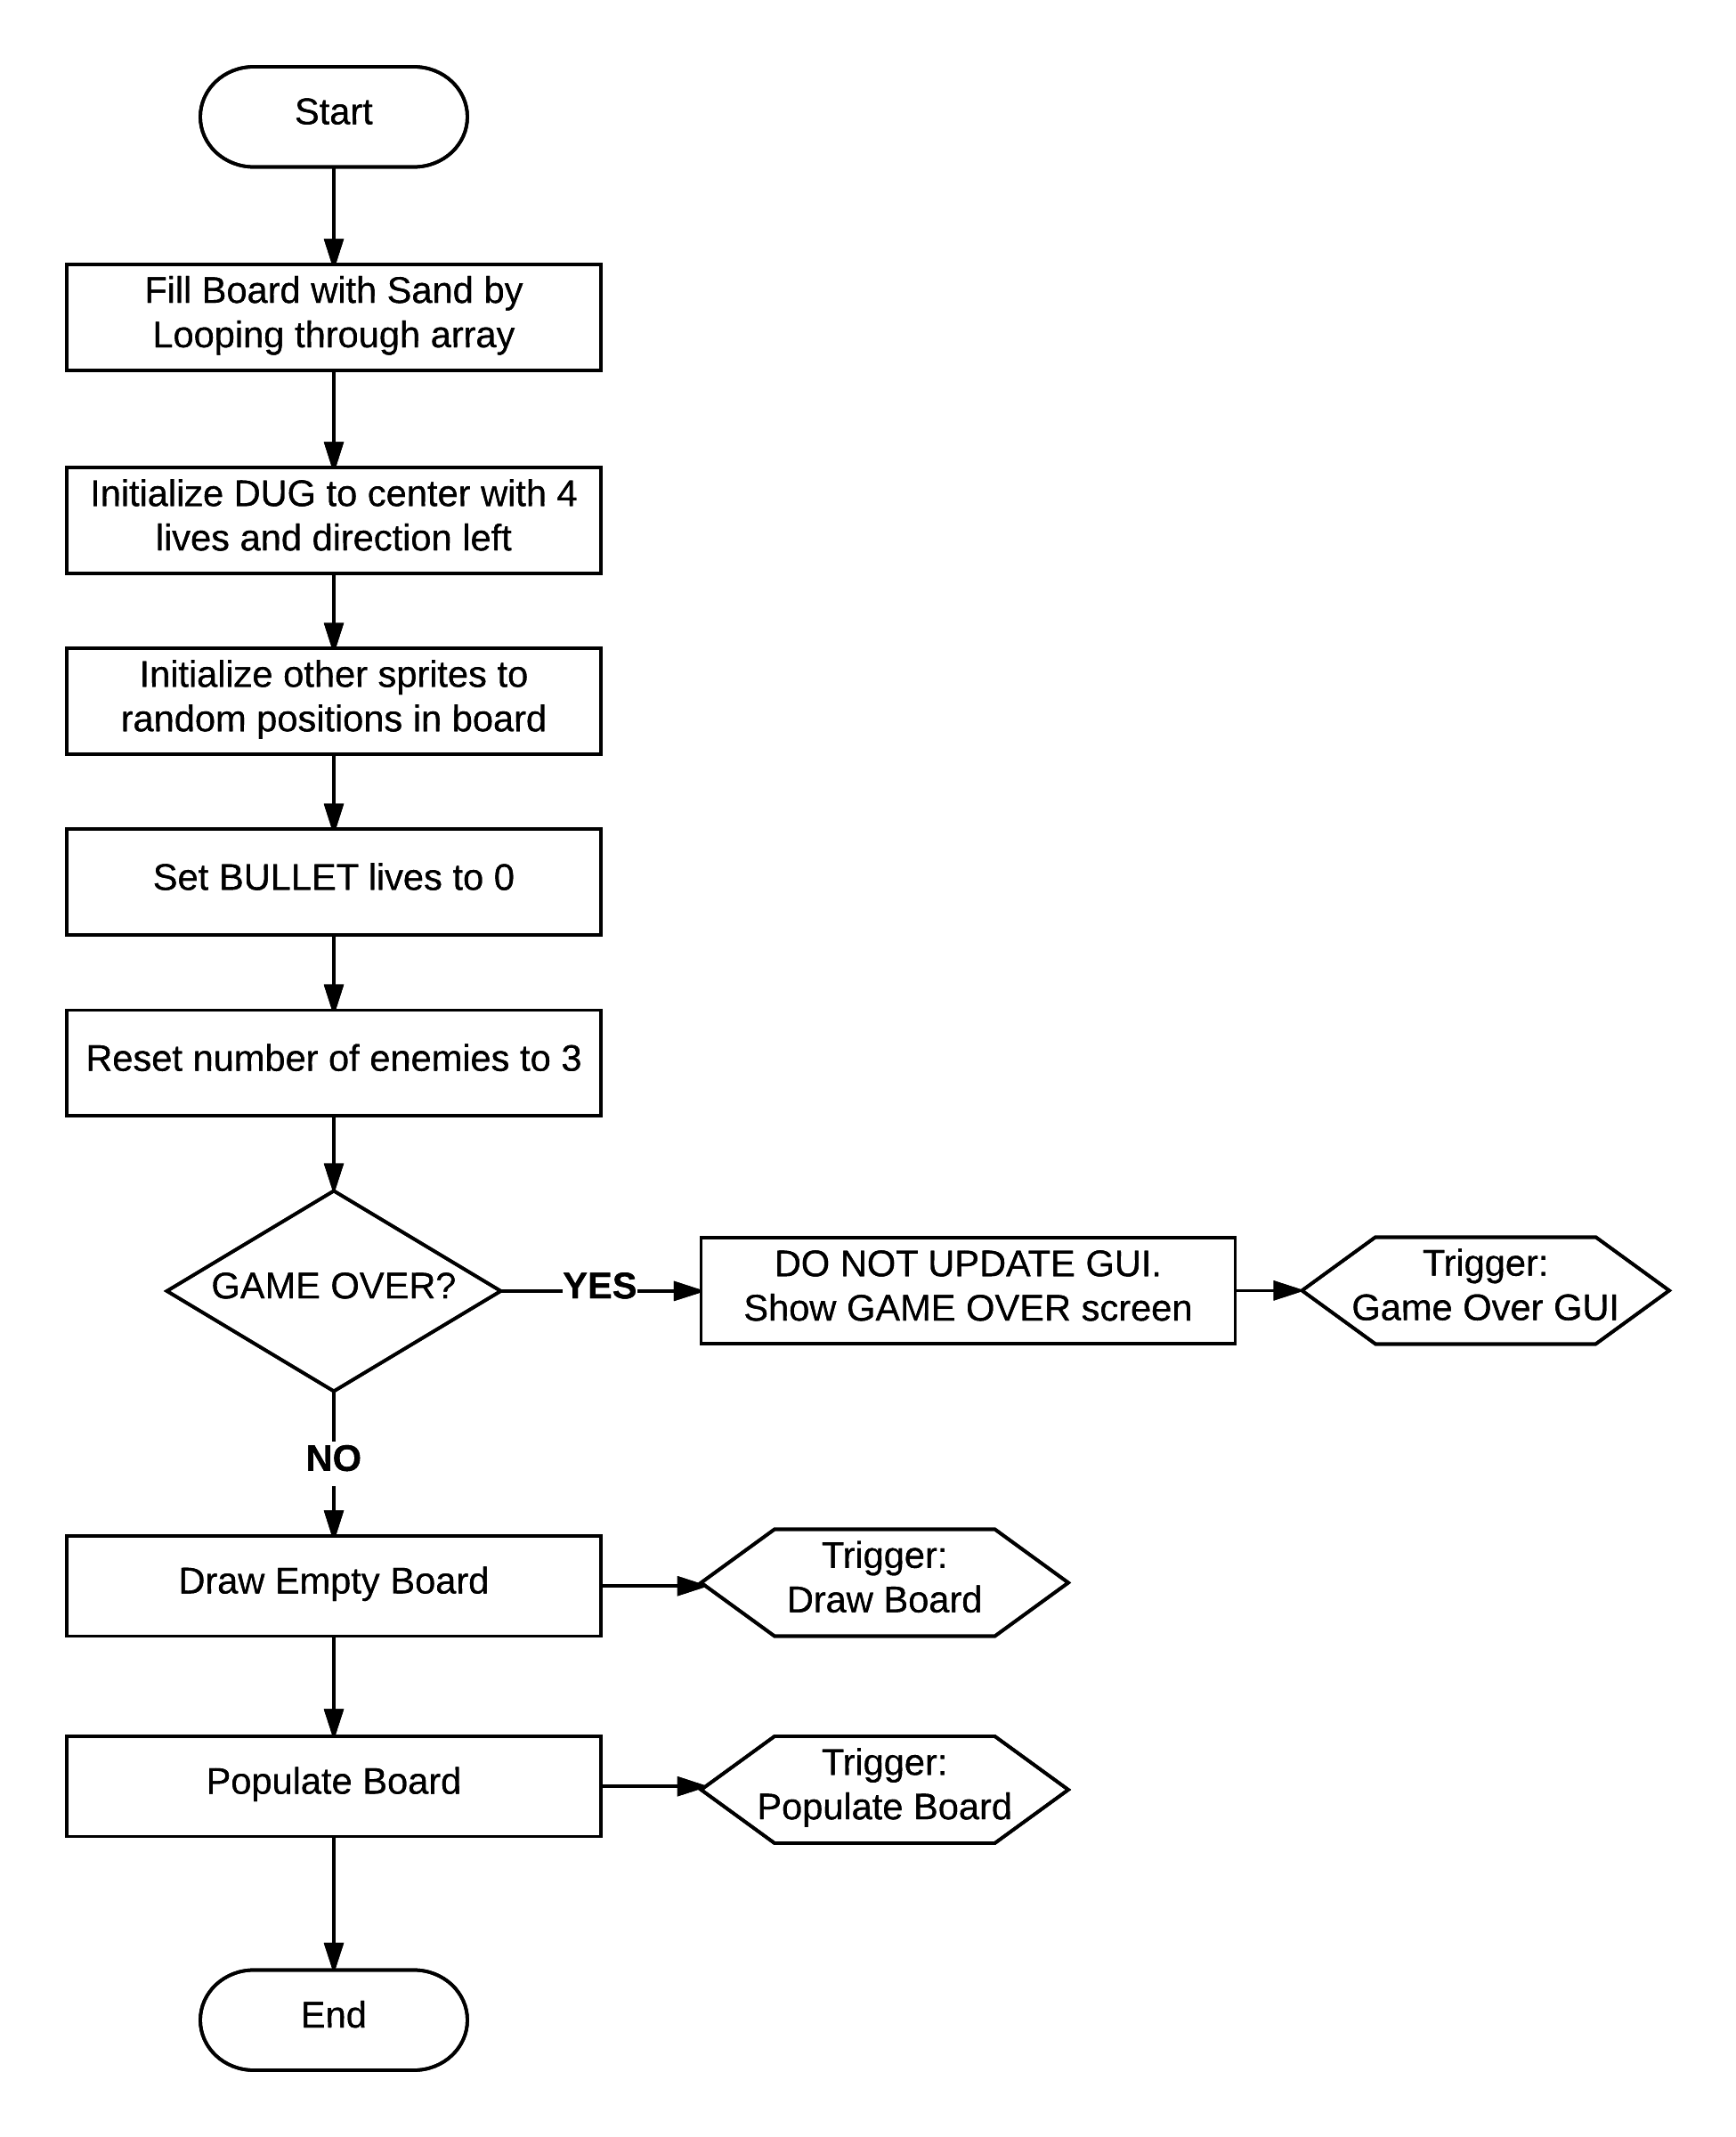
\includegraphics[width=0.9\textwidth]{images/reset-model.png}
      \caption{\label{fig:reset-model} Reset Model Flowchart}
    \end{figure}

    \textbf{Model} is initialized by setting the \texttt{CURRENT SCORE} to \texttt{0} and \texttt{LEVEL} to \texttt{1}.

    Then the \textbf{Model} is separately reset, that is, it resets the position of the sprites, refills the board with sand and prepares the game to be played.
    The \textbf{Model} is reset in 2 instances, when the game is initialized at boot up, and when the \textbf{Model} is in the \texttt{GAME OVER} state.

    \subsubsection{Game States and Representation}

    There are 4 variables that describe the \textbf{Model}'s state. These are:

    \begin{table}[H]
      \begin{tabular}{ll}
	\texttt{BEGIN\_GAME}	&   True if we need the game to begin from the instructions screen. \\
	\texttt{RUNNING\_P}	&   This tells us whether the game is running or not. This is 1 when the game is running. \\
	\texttt{PAUSE\_GAME}	&   If the game is not running and this flag is up, the game is in the \texttt{PAUSED} state.\\
	\texttt{GAME\_OVER}	&   When the game is not running and this flag is up, the game is in the \texttt{GAME OVER} state.
      \end{tabular}
    \end{table}

    For each state, model is updated differently. If game is not \texttt{RUNNING} the model isn't updated and the appropriate subroutine call is made to handle either \texttt{PAUSED} or \texttt{GAME OVER} state, where the GUI is updated to show the state.

    \subsubsection{Update Model and Control Sprites}

    \begin{figure}[H]
      \centering
      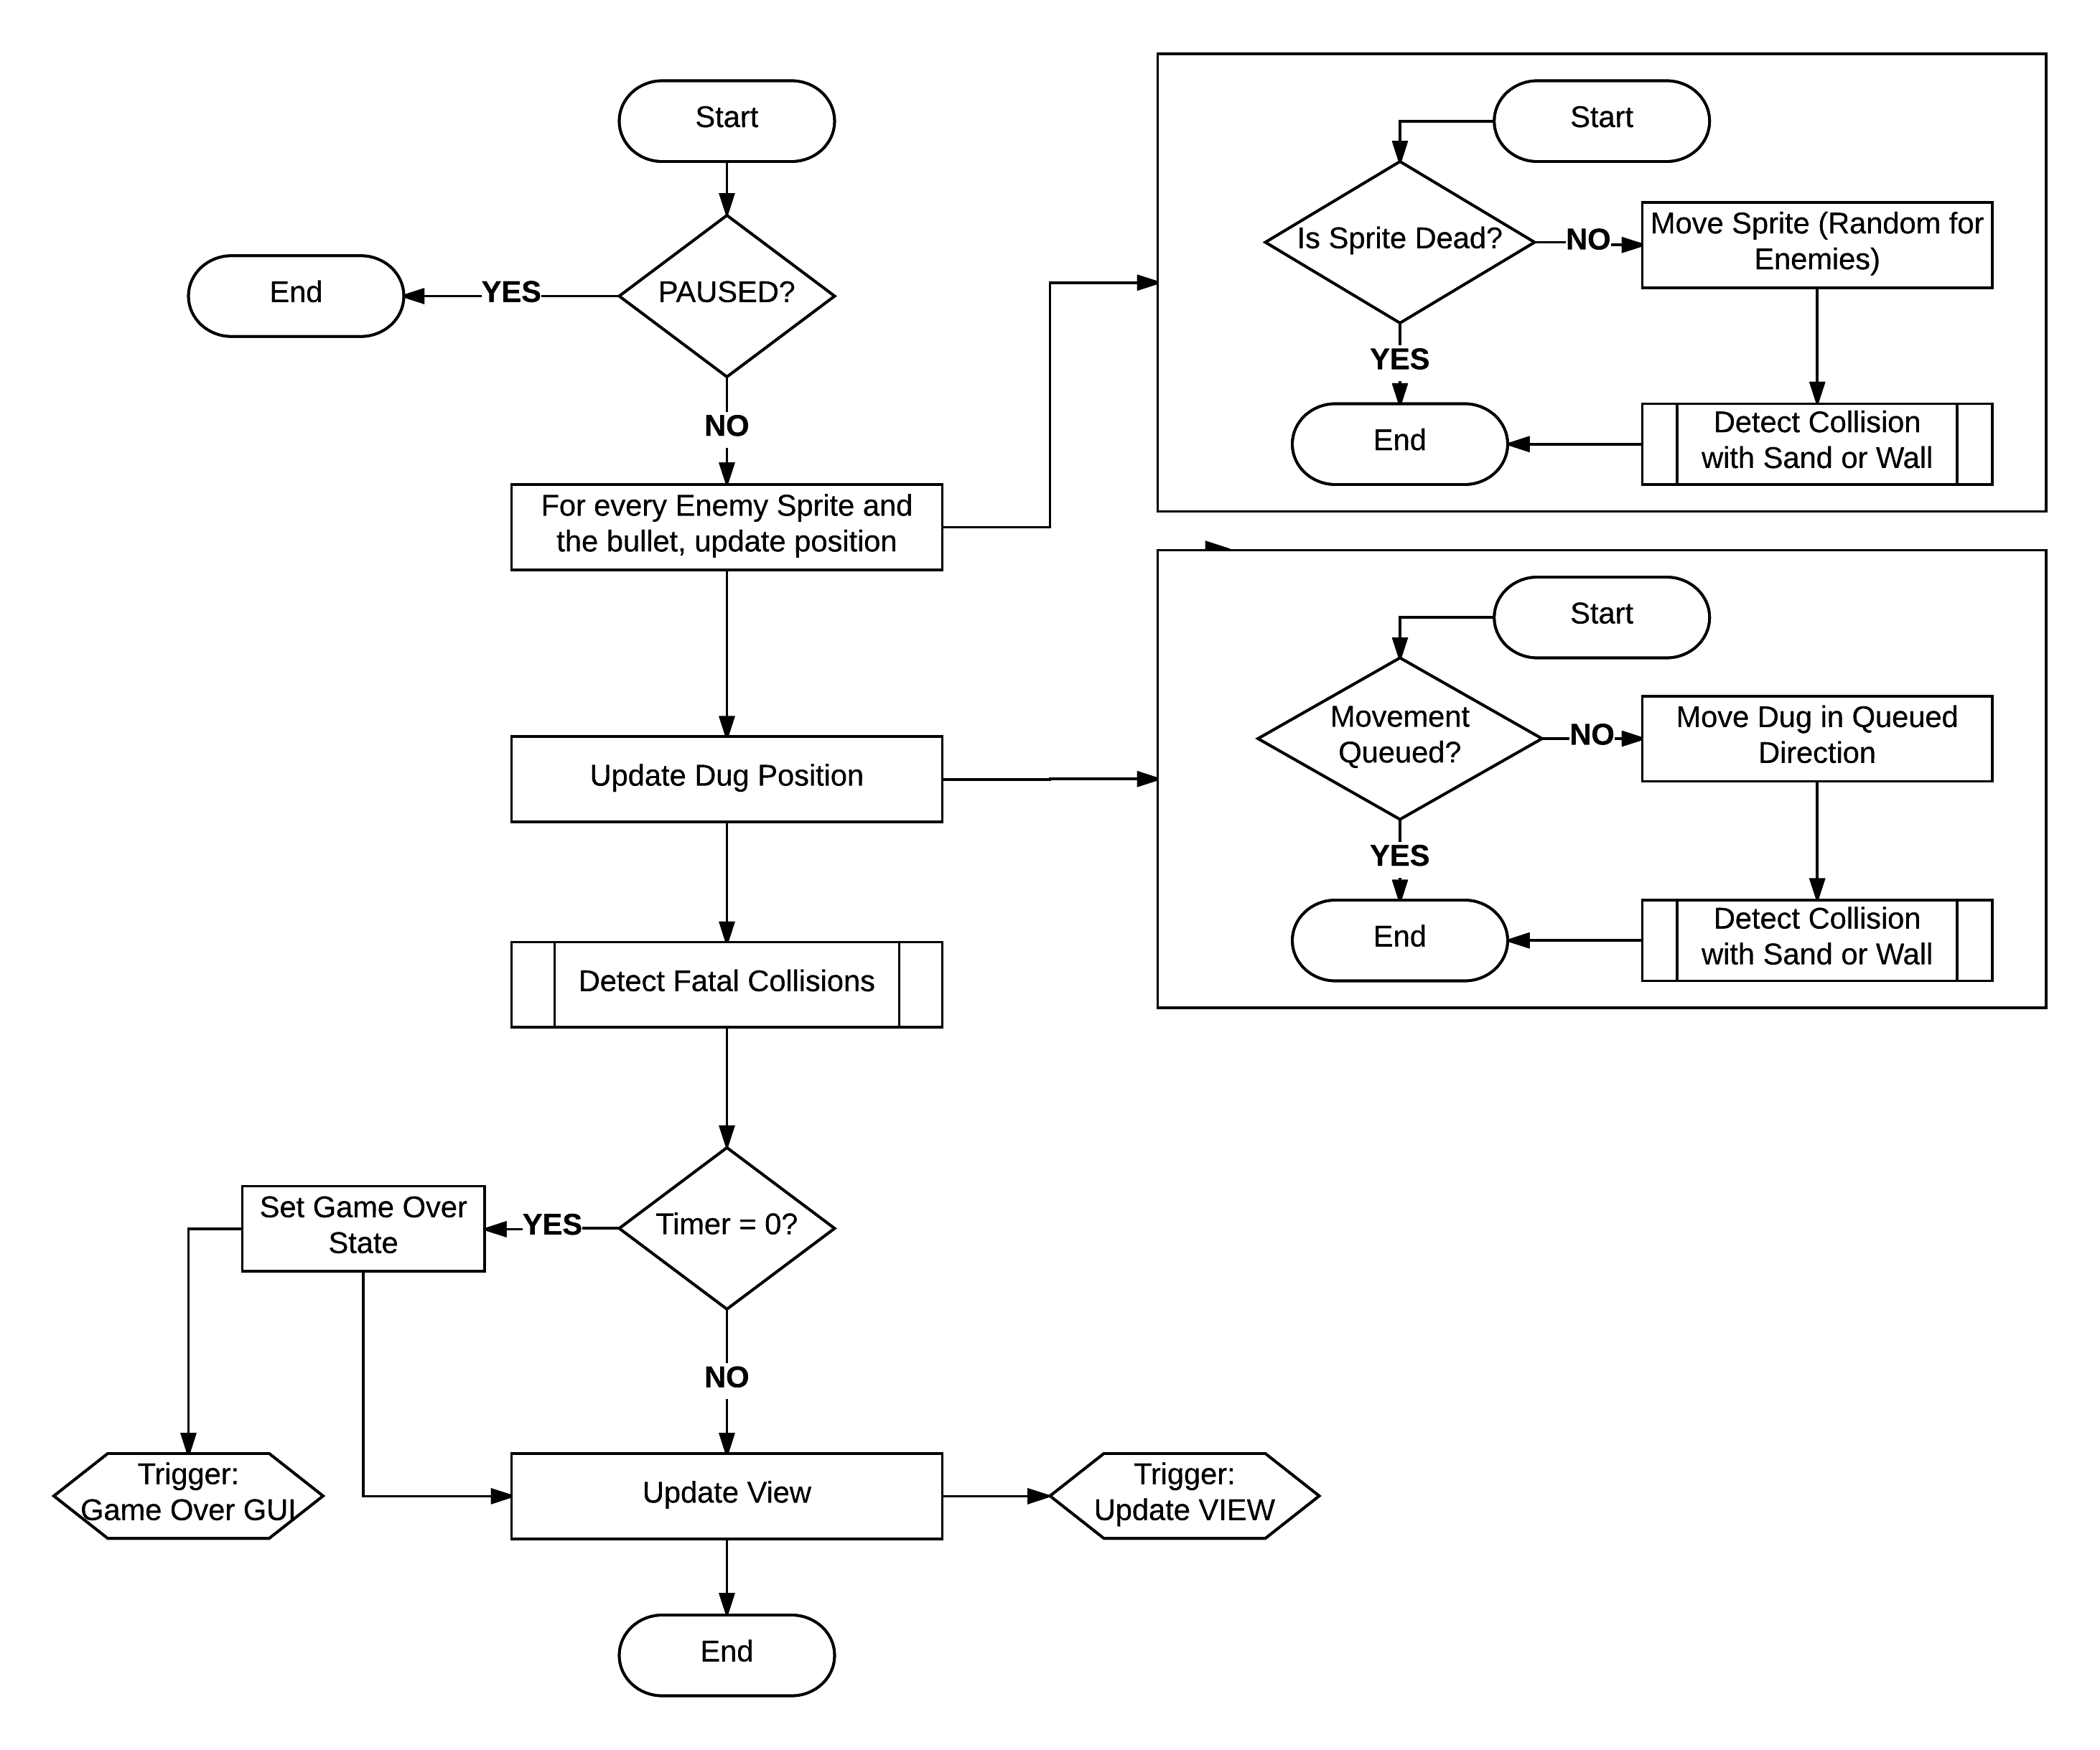
\includegraphics[width=0.9\textwidth]{images/update-model.png}
      \caption{\label{fig:update-model} Update Model Flowsheet}

    \end{figure}

    \subsubsection{Collision Detection}

    Collision detection is the main component of the \textbf{Model}. This is because there are 2 possible outcomes from each collisions, and because of the nature of the game, there are 2 ways collisions can happen.

    But first, let us discuss the outcomes for each collision and how it differs depending on the involved sprites/objects.

    \subsubsection*{Fatal Outcome}

    Fatal outcomes are those outcomes in which the victim sprite loses a life when it collides with another sprite or object. Depending on the victim sprite, the attacking sprite can differ.
    The following is a mapping from type of sprite to sprites/objects that are fatal to it, along with any other outcomes:

    \begin{tabular}{clcll}
      $\bullet$ & Enemies	& -- &  Bullet		&   $\rightarrow$ Points for killing enemy \\
      $\bullet$ & Bullet	& -- &  Sand, Wall, Enemy	&   $\rightarrow$ Nothing \\
      $\bullet$ & Dug		& -- &  Enemy		&   $\rightarrow$ GAME OVER if Dug has 0 lives
    \end{tabular}

    \subsubsection*{Non-Fatal Outcome}

    Non-fatal outcomes are those in which the victim sprite does not lose a life during the collision. The outcomes differ based on the sprites involved in the collision.
    The following are all possible non-fatal collisions between two types of sprites/objects, with the outcome of the collision:

    \begin{tabular}{clcll}
      $\bullet$ & Enemies   & -- &  Enemies &	$\rightarrow$ Nothing\\
      $\bullet$ & Enemies   & -- &  Wall/Sand &	$\rightarrow$ Enemy sprite chooses a random free path around it and heads along that.\\
      $\bullet$ & Dug   & -- &  Wall &	$\rightarrow$ Nothing.\\
      $\bullet$ & Dug   & -- & Sand &	$\rightarrow$ Gain 10 points.\\
    \end{tabular}


  Now, let us discuss the types of collisions between moving sprites. These are 2 scenarios, \textbf{Type 1}, where the two sprites are on the same spot, or \textbf{Type 2}, where the sprites were right next to each other in the previous frame and pass each other in the next one. The second one is the more challenging type and occurs when the two sprites are on a head-on collision while being right next to each other. By the nature of fram updates, the sprites don't land on the same coordinate.

  \subsubsection*{Type 1: Sprites arrive on the same Coordinate}

  This is the easy case, when the sprites arrive on the same spot. This is the more common case and can be detected by just checking if the two sprites have the same X and Y coordinate.

  \subsubsection*{Type 2: Sprites do not arrive on the same Coordinate}

  This happens when sprites do not arrive on the same position when on a head-on collision course. This scenario can be shown easily with the following illustration:

  \begin{table}[H]
    \centering
  \begin{tabular}{|l|cccc|}

    \hline
    Frame 1 &	$>$ &	.   &	.   &	$<$ \\ \hline
    Frame 2 &	.   &	$>$ &	$<$ & .	    \\ \hline
    Present Frame &	.   &	$<$ &	$>$ & .	    \\ \hline

  \end{tabular}
  \\[5pt]
  Here, $>$ and $<$ are sprites moving towards each other
  \end{table}

  This can be detected by checking the following:

  \begin{itemize}
    \item \texttt{SPRITE 1}'s current position and \texttt{SPRITE 2}'s old position are same.
    \item \texttt{SPRITE 2}'s current position and \texttt{SPRITE 1}'s old position are same.
    \item If both of the above are \texttt{TRUE}, the collision is fatal.
  \end{itemize}
